\section{Theory}
The experiment is based on the opto-magnetic property, demonstrating Faraday effect which states that isotropic media become optically active when a magnetic field is applied in the propagation direction of the light. A linearly polarised light propagating along the $x$ direction can be expressed as a superposition of left and right circularly polarised components.
\begin{equation}
    \vb{E}(x,t) = \vb{E}\tund{r}(x,t) + \vb{E}\tund{l}(x,t)
\end{equation}
where $\vb{E}\tund{r}$ and $\vb{E}\tund{l}$ denote the left and right circular components. Written explicitly we have, 
\begin{align}
    \begin{split}
         \vb{E}\tund{r}(x,t) &= \qty(0, \frac{A}{2}\cos \qty[\omega\qty(t-n\tund{r}x/c)], \frac{A}{2}\sin \qty[\omega\qty(t-n\tund{r}x/c)])^\top\\
    \vb{E}\tund{l}(x,t) &= \qty(0, \frac{A}{2}\cos \qty[\omega\qty(t-n\tund{r}x/c)], -\frac{A}{2}\sin \qty[\omega\qty(t-n\tund{r}x/c)])^\top
    \end{split}
\end{align}
where $n\tund{r}$ and $n\tund{l}$ are the different refractive indices for the RCP and LCP components. Let us choose $x=D$, and using the above relation we will obtain: 
\begin{align}
    \psi= \tan^{-1}\qty(\frac{E\tund{z}}{E\tund{y}}) = \frac{\omega}{2c}(n\tund{l}-n\tund{r})D\implies \psi = (n\tund{l}-n\tund{r}) \frac{\pi D}{\lambda}
\end{align}
This shows that the difference in the refractive indices can rotate the linearly polarised light. Now, we show that the introduction of a magnetic field will change the refractive index for the two polarisation components using Becquerel's theory.\\[0.2cm] Consider a material containing particles of mass $m$ and charge $q$, embedded in an opposite charge distribution. The system can be modelled as the masses being contrained by springs and vibrating about fixed sites. Considering magnetic field along the $x$ axis and a plane RCP rotating clockwise with respect to the field, the equation of motion can be written as, 
\begin{equation}
    -m\omega^2 r\tund{rcp} = -kr + Eq +Bq\omega r \implies r = \frac{Eq/m}{(\omega\tund{0}^2 - \omega^2-Bq\omega)}
\end{equation}
where $\omega\tund{0}^2 = \qty(\frac{k}{m})^{1/2}$ to be the natural frequency. Similarly, for the left circularly polarised light we can find, 
\begin{equation}
    r\tund{lcp} = \frac{Eq/m}{(\omega\tund{0}^2 -\omega^2+Bq\omega)}
\end{equation}
\begin{figure}[H]
    \centering


\tikzset{every picture/.style={line width=0.75pt}} %set default line width to 0.75pt        

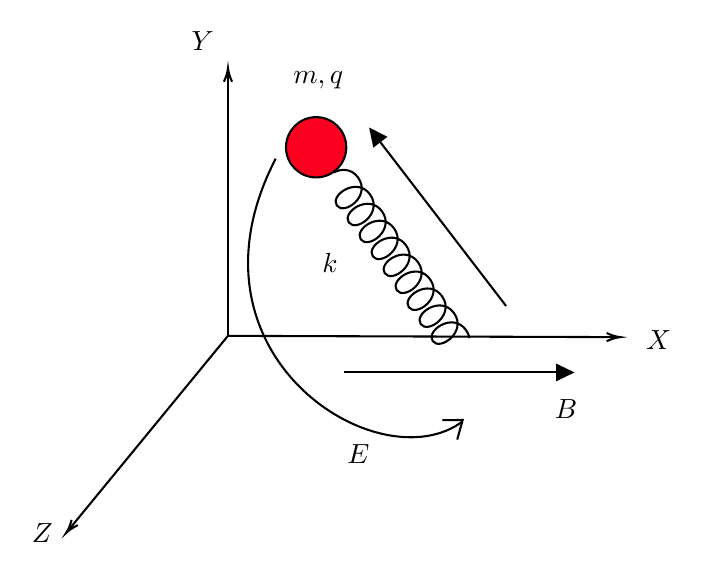
\begin{tikzpicture}[x=0.75pt,y=0.75pt,yscale=-1,xscale=1]
%uncomment if require: \path (0,300); %set diagram left start at 0, and has height of 300

%Straight Lines [id:da587631839804891] 
\draw    (263,169.38) -- (450,169.99) ;
\draw [shift={(452,170)}, rotate = 180.19] [color={rgb, 255:red, 0; green, 0; blue, 0 }  ][line width=0.75]    (6.56,-1.97) .. controls (4.17,-0.84) and (1.99,-0.18) .. (0,0) .. controls (1.99,0.18) and (4.17,0.84) .. (6.56,1.97)   ;
%Straight Lines [id:da12065738469387544] 
\draw    (263,169.38) -- (263,42.38) ;
\draw [shift={(263,40.38)}, rotate = 90] [color={rgb, 255:red, 0; green, 0; blue, 0 }  ][line width=0.75]    (6.56,-1.97) .. controls (4.17,-0.84) and (1.99,-0.18) .. (0,0) .. controls (1.99,0.18) and (4.17,0.84) .. (6.56,1.97)   ;
%Straight Lines [id:da30395749047798737] 
\draw    (263,169.38) -- (186.27,262.84) ;
\draw [shift={(185,264.38)}, rotate = 309.39] [color={rgb, 255:red, 0; green, 0; blue, 0 }  ][line width=0.75]    (6.56,-1.97) .. controls (4.17,-0.84) and (1.99,-0.18) .. (0,0) .. controls (1.99,0.18) and (4.17,0.84) .. (6.56,1.97)   ;
%Shape: Spring [id:dp5902213662742808] 
\draw   (314.01,90.58) .. controls (317.67,88.76) and (322.56,88.67) .. (325.73,93.16) .. controls (332.09,102.14) and (318.9,111.47) .. (315.44,106.57) .. controls (311.97,101.67) and (325.15,92.35) .. (331.51,101.33) .. controls (337.86,110.31) and (324.68,119.63) .. (321.21,114.74) .. controls (317.75,109.84) and (330.93,100.51) .. (337.28,109.49) .. controls (343.64,118.47) and (330.45,127.8) .. (326.99,122.9) .. controls (323.52,118) and (336.71,108.67) .. (343.06,117.65) .. controls (349.41,126.63) and (336.23,135.96) .. (332.76,131.06) .. controls (329.3,126.16) and (342.48,116.84) .. (348.83,125.82) .. controls (355.19,134.8) and (342,144.12) .. (338.54,139.23) .. controls (335.07,134.33) and (348.26,125) .. (354.61,133.98) .. controls (360.96,142.96) and (347.78,152.29) .. (344.31,147.39) .. controls (340.85,142.49) and (354.03,133.16) .. (360.39,142.14) .. controls (366.74,151.12) and (353.56,160.45) .. (350.09,155.55) .. controls (346.63,150.65) and (359.81,141.33) .. (366.16,150.31) .. controls (372.52,159.29) and (359.33,168.61) .. (355.87,163.72) .. controls (352.4,158.82) and (365.58,149.49) .. (371.94,158.47) .. controls (378.29,167.45) and (365.11,176.78) .. (361.64,171.88) .. controls (358.18,166.98) and (371.36,157.65) .. (377.71,166.63) .. controls (378.61,167.9) and (379.12,169.18) .. (379.32,170.43) ;
%Shape: Circle [id:dp24368971639430537] 
\draw  [fill={rgb, 255:red, 252; green, 0; blue, 31 }  ,fill opacity=1 ] (290.95,78.53) .. controls (290.95,70.5) and (297.45,64) .. (305.47,64) .. controls (313.5,64) and (320,70.5) .. (320,78.53) .. controls (320,86.55) and (313.5,93.05) .. (305.47,93.05) .. controls (297.45,93.05) and (290.95,86.55) .. (290.95,78.53) -- cycle ;
%Curve Lines [id:da7312278265824699] 
\draw    (286,84) .. controls (237,178.62) and (336,240.62) .. (376,210.62) ;
\draw   (366.28,209.97) -- (376.07,209.92) -- (373.45,219.34) ;
%Straight Lines [id:da47516934334617367] 
\draw    (332.83,71.38) -- (397,155) ;
\draw [shift={(331,69)}, rotate = 52.5] [fill={rgb, 255:red, 0; green, 0; blue, 0 }  ][line width=0.08]  [draw opacity=0] (8.93,-4.29) -- (0,0) -- (8.93,4.29) -- cycle    ;
%Straight Lines [id:da2931732983365879] 
\draw    (427,187) -- (319,187) ;
\draw [shift={(430,187)}, rotate = 180] [fill={rgb, 255:red, 0; green, 0; blue, 0 }  ][line width=0.08]  [draw opacity=0] (8.93,-4.29) -- (0,0) -- (8.93,4.29) -- cycle    ;

% Text Node
\draw (293,40.4) node [anchor=north west][inner sep=0.75pt]    {$m,q$};
% Text Node
\draw (419,198.4) node [anchor=north west][inner sep=0.75pt]    {$B$};
% Text Node
\draw (319,220.4) node [anchor=north west][inner sep=0.75pt]    {$E$};
% Text Node
\draw (307,128.2) node [anchor=north west][inner sep=0.75pt]    {$k$};
% Text Node
\draw (463,165.4) node [anchor=north west][inner sep=0.75pt]    {$X$};
% Text Node
\draw (244,21.4) node [anchor=north west][inner sep=0.75pt]    {$Y$};
% Text Node
\draw (167,258.4) node [anchor=north west][inner sep=0.75pt]    {$Z$};


\end{tikzpicture}

\end{figure}
\noindent
The displacement of the charge creates a dipole moment $qr$. Suppose there are $N$ dipoles per volume in the system. Then the polarisation per volume is given by $P=Nqr$. Considering linear polarisation, $P = \varepsilon\tund{0}\chi\tund{e}E$ where $ \varepsilon\tund{0}$ is the permittivity of the free space and $\chi\tund{e}$ is the electric susceptibility. Now, the relative permittivity is, $\varepsilon\tund{r} = \chi\tund{e}+1 = 1+\frac{P}{\chi\tund{0}E}$. From the value of the relative permittivity $n=\sqrt{\varepsilon\tund{r}\mu\tund{r}}$. Taking $\mu\tund{r} =1$,  we get:
\begin{align}
    \begin{split}
        n\tund{r}(\omega) &= \qty[1+\frac{Nq^2}{m\qty(\omega\tund{0}^2 -\omega^2-\frac{Bq\omega}{m})}]^{1/2}\\
    n\tund{l}(\omega) &= \qty[1+\frac{Nq^2}{m\qty(\omega\tund{0}^2 -\omega^2+\frac{Bq\omega}{m})}]^{1/2}
    \end{split}
\end{align}
\noindent
Considering the approximation, $\omega^2 + \frac{Bq\omega}{m} = (\omega + \Delta \omega\tund{r})^2$ and $\omega^2 -\frac{Bq\omega}{m}= (\omega+\Delta \omega\tund{l})^2$ where $\Delta \omega\tund{r} = -\Delta \omega\tund{l}= \frac{Bq}{2m}$ is considered to be small, we get:
\begin{align}
    n\tund{l} - n\tund{r} = \dv{n}{\omega}\cdot (\Delta \omega\tund{l} -\Delta \omega\tund{r} ) = \dv{n}{\lambda}\cdot \dv{\lambda}{\omega} \cdot \qty(-\frac{Bq}{m})= \dv{n}{\lambda}\cdot \qty(\frac{\lambda^2}{2\pi c})\cdot \qty(\frac{Bq}{m})
\end{align}
This implies that the optical rotation can be written, $\Psi =  VDB$ where $V$ is the Verdet constant, 
\begin{align}
    V = \dv{n}{\lambda}\cdot \frac{\lambda}{2c}\cdot \frac{q}{m}
\end{align}
The figure below shows the setup which we used for our experiments, along with all the optical elements.
\begin{figure}[H]
    \centering
% Pattern Info
 
\tikzset{
pattern size/.store in=\mcSize, 
pattern size = 5pt,
pattern thickness/.store in=\mcThickness, 
pattern thickness = 0.3pt,
pattern radius/.store in=\mcRadius, 
pattern radius = 1pt}
\makeatletter
\pgfutil@ifundefined{pgf@pattern@name@_bogd6fx0k}{
\pgfdeclarepatternformonly[\mcThickness,\mcSize]{_bogd6fx0k}
{\pgfqpoint{0pt}{0pt}}
{\pgfpoint{\mcSize+\mcThickness}{\mcSize+\mcThickness}}
{\pgfpoint{\mcSize}{\mcSize}}
{
\pgfsetcolor{\tikz@pattern@color}
\pgfsetlinewidth{\mcThickness}
\pgfpathmoveto{\pgfqpoint{0pt}{0pt}}
\pgfpathlineto{\pgfpoint{\mcSize+\mcThickness}{\mcSize+\mcThickness}}
\pgfusepath{stroke}
}}
\makeatother
\tikzset{every picture/.style={line width=0.75pt}} %set default line width to 0.75pt        

\begin{tikzpicture}[x=0.75pt,y=0.75pt,yscale=-1,xscale=1]
%uncomment if require: \path (0,371); %set diagram left start at 0, and has height of 371

%Shape: Path Data [id:dp8664686596982926] 
\draw  [fill={rgb, 255:red, 255; green, 34; blue, 34 }  ,fill opacity=1 ] (144,71) -- (144,59.95) -- (171.91,59.95) -- (181,65.47) -- (171.91,71) -- (144,71) -- cycle ;
%Straight Lines [id:da802081735087196] 
\draw  [dash pattern={on 4.5pt off 4.5pt}]  (316.94,65.28) -- (401,65.17) ;
%Shape: Ellipse [id:dp5889281662699898] 
\draw  [fill={rgb, 255:red, 247; green, 237; blue, 157 }  ,fill opacity=1 ] (349,87) .. controls (343.48,87) and (339,77.07) .. (339,64.82) .. controls (339,52.57) and (343.48,42.63) .. (349,42.63) .. controls (354.52,42.63) and (359,52.57) .. (359,64.82) .. controls (359,77.07) and (354.52,87) .. (349,87) -- cycle ;
%Shape: Rectangle [id:dp36016788018664725] 
\draw  [pattern=_bogd6fx0k,pattern size=6pt,pattern thickness=0.75pt,pattern radius=0pt, pattern color={rgb, 255:red, 0; green, 0; blue, 0}] (401,34) -- (408,34) -- (408,93.18) -- (401,93.18) -- cycle ;
%Shape: Inductor (Air Core) [id:dp6064016736188501] 
\draw   (283.94,65.28) -- (289.88,65.28) .. controls (289.97,62.95) and (290.79,60.95) .. (291.96,60.26) .. controls (293.12,59.56) and (294.4,60.3) .. (295.16,62.13) .. controls (295.75,63.55) and (295.99,65.39) .. (295.82,67.18) .. controls (295.82,67.87) and (295.52,68.44) .. (295.16,68.44) .. controls (294.8,68.44) and (294.5,67.87) .. (294.5,67.18) .. controls (294.33,65.39) and (294.57,63.55) .. (295.16,62.13) .. controls (295.85,60.61) and (296.8,59.75) .. (297.8,59.75) .. controls (298.8,59.75) and (299.75,60.61) .. (300.44,62.13) .. controls (301.03,63.55) and (301.27,65.39) .. (301.1,67.18) .. controls (301.1,67.87) and (300.8,68.44) .. (300.44,68.44) .. controls (300.08,68.44) and (299.78,67.87) .. (299.78,67.18) .. controls (299.61,65.39) and (299.85,63.55) .. (300.44,62.13) .. controls (301.13,60.61) and (302.08,59.75) .. (303.08,59.75) .. controls (304.08,59.75) and (305.03,60.61) .. (305.72,62.13) .. controls (306.31,63.55) and (306.55,65.39) .. (306.38,67.18) .. controls (306.38,67.87) and (306.08,68.44) .. (305.72,68.44) .. controls (305.36,68.44) and (305.06,67.87) .. (305.06,67.18) .. controls (304.89,65.39) and (305.13,63.55) .. (305.72,62.13) .. controls (306.48,60.3) and (307.76,59.56) .. (308.92,60.26) .. controls (310.09,60.95) and (310.91,62.95) .. (311,65.28) -- (316.94,65.28) ;
%Shape: Path Data [id:dp36291327620802716] 
\draw  [fill={rgb, 255:red, 80; green, 227; blue, 194 }  ,fill opacity=1 ] (317,51.78) -- (317,76.78) -- (284,76.78) -- (284,51.78) -- (317,51.78) -- cycle (282,49.26) -- (282,79.31) -- (319,79.31) -- (319,49.26) -- (282,49.26) -- cycle ;
%Straight Lines [id:da039821981068300594] 
\draw  [dash pattern={on 4.5pt off 4.5pt}]  (181,65.47) -- (283.94,65.28) ;
%Shape: Ellipse [id:dp311819918000398] 
\draw  [fill={rgb, 255:red, 247; green, 237; blue, 157 }  ,fill opacity=1 ] (242,86.83) .. controls (236.48,86.83) and (232,76.9) .. (232,64.65) .. controls (232,52.4) and (236.48,42.47) .. (242,42.47) .. controls (247.52,42.47) and (252,52.4) .. (252,64.65) .. controls (252,76.9) and (247.52,86.83) .. (242,86.83) -- cycle ;

% Text Node
\draw (143,77) node [anchor=north west][inner sep=0.75pt]  [font=\scriptsize] [align=left] {Laser};
% Text Node
\draw (206,26.83) node [anchor=north west][inner sep=0.75pt]  [font=\scriptsize] [align=left] {Polarizer $\displaystyle P_{1}$};
% Text Node
\draw (321,27) node [anchor=north west][inner sep=0.75pt]  [font=\scriptsize] [align=left] {Polarizer $\displaystyle P_{2}$};
% Text Node
\draw (411,82.18) node [anchor=north west][inner sep=0.75pt]  [font=\scriptsize,rotate=-270] [align=left] {Detector};
% Text Node
\draw (266,85) node [anchor=north west][inner sep=0.75pt]  [font=\scriptsize] [align=left] {Electromagnet};


\end{tikzpicture}
\caption{Schematic of the Experimental Setup}
\end{figure}
\begin{figure}[H]
    \centering
    
\includegraphics[width=0.5\textwidth]{setup.jpeg}
    \caption{Actual experimental setup}
\end{figure}
We also verify Malu's law, which states $\mathcal{I} = \mathcal{I}\tund{0}\cos^2(\Psi)$ and $\Psi$ is proportional to the current $I$. For small values of optical rotation, we have a quadratic relation between intensity and current, $\mathcal{I} \sim I^2$.